\documentclass[10pt,a4paper]{article}
\usepackage{tikz} % for drawing figures
\usepackage{amsmath} % for equations
\usepackage{url} % for URLs
\usepackage{graphicx}
\usepackage{multicol}
\usepackage{varwidth}
\usepackage{blindtext}


\usepackage{linguex} % ** special include in directory: for doing handy example labeling and bracketing
\renewcommand{\firstrefdash}{} % used for linguex package not to put hyphens in example refs (1a instead of 1-a)
\usepackage{cogsci}
\usepackage{pslatex}
\usepackage{apacite}

\newcommand{\sem}[1]{\mbox{$[\![$#1$]\!]$}}
\newcommand{\lam}{$\lambda$}
\newcommand{\gcs}[1]{\textcolor{blue}{[gcs: #1]}} 



\title{Subjectivity-based adjective ordering maximizes the probability of successful reference resolution}
\author{\large \textbf{our names}\\
our emails\\
our affiliations}


\begin{document}
\maketitle

\begin{abstract}
Adjective ordering preferences (e.g., \emph{big blue box} vs.~\emph{blue big box}) are robustly attested in English and many unrelated languages \cite{dixon1982}. \citeA{scontrasetal2017adjectives} showed that adjective subjectivity is a robust predictor of ordering preferences in English: less subjective adjectives are preferred closer to the modified noun. In a follow-up to this empirical finding, \citeA{simonic2018} and \citeauthor{scontrasetalSPadjectives} (to appear) claim that pressures from successful reference resolution and the hierarchical structure of modification explain subjectivity-based ordering preferences. We provide further support for this claim using large-scale simulations of reference scenarios, together with an empirically-motivated adjective semantics. In the vast majority of cases, subjectivity-based adjective orderings yield a higher probability of successful reference resolution.


\textbf{Keywords:} 
adjective ordering, subjectivity, reference resolution, hierarchical modification

\end{abstract}

\section{Introduction}

When speakers use two or more adjectives to modify a noun, they exhibit robust preferences in the relative order of the adjectives (e.g., \emph{big blue box} vs.~\emph{blue big box}). These preferences surface also in listeners as they encounter multi-adjective strings. Using a series of behavioral and corpus experiments, \citeA{scontrasetal2017adjectives} demonstrated that adjective order in multi-adjective strings is reliably predicted by the subjectivity of the adjectives involved: less subjective adjectives are preferred closer to the modified noun, and the strength of the preference is modulated by the subjectivity differential between the adjectives. Thus, speakers and listeners strongly prefer \emph{big blue box} over \emph{blue big box}, as \emph{blue} is much less subjective than \emph{big}.

The question that immediately arises is why subjectivity should play the role it does in adjective ordering preferences. The current work follows \citeA{simonic2018} and \citeauthor{scontrasetalSPadjectives} (to appear) in advancing the claim that pressures from successful reference resolution deliver subjectivity-based ordering preferences. In cases of restrictive modification, adjectives that compose with the nominal later will classify a smaller set of potential referents (e.g., the set of boxes vs. the set of blue boxes). To avoid alignment errors where a listener might mis-characterize the intended referent, speakers introduce the more error-prone (i.e., more subjective) adjectives later in the hierarchical construction of nominal structure where they operate over a restricted set of potential referents; the structure linearizes such that subjectivity decreases the closer you get to the modified noun. 
We build on the work that precedes ours by making minimal assumptions about online processing (cf.~\citeauthor{scontrasetalSPadjectives}, to appear) and by assuming a more principled implementation of adjective subjectivity within an empirically-motivated semantics (cf.~\citeNP{simonic2018}).

The paper is structured as follows. First, we review the empirical generalization concerning subjectivity-based preferences, together with the proposals offered to account for this generalization. Then, we consider empirical work on adjective semantics, which serves as inspiration for our own proposal. We demonstrate how a minimal set of independently-motivated assumptions leads to a ready explanation for subjectivity-based ordering preferences: ordering adjectives with respect to decreasing subjectivity maximizes the probability of successful reference resolution. We conclude by considering how knowledge of these preferences might get represented in the minds of language users.



\section{Background}

Given the robustness of adjective ordering preferences within and across languages, there has been no shortage of proposals meant to account for the regularities in adjective ordering. Some have offered grammatical proposals that attend to semantic composition or articulated syntactic hierarchies (e.g., \citeNP{cinque1994,scott2002,mcnallyboleda2004,truswell2009}). Others have advanced more psychological proposals built around notions like inherentness or accessibility (e.g, \citeNP{whorf1945,ziff1960,martin1969}). Recently, \citeA{scontrasetal2017adjectives} synthesized several proposals that preceded them and advanced the hypothesis that adjective subjectivity predicts ordering preferences (see also \citeNP{quirketal1985,hetzron1978,dixon1982,tucker1998,hill2012}). 

In order to test the subjectivity hypothesis, \citeauthor{scontrasetal2017adjectives} first had to determine what the ordering preferences were. They established a behavioral measure of the preferences whereby experimental participants indicated the preferred ordering of multi-adjective strings that differed only in the relative order of the adjectives involved (e.g., \emph{the big blue box} vs. \emph{the blue big box}). \citeauthor{scontrasetal2017adjectives} then validated their behavioral measure by comparing it with naturalistic productions from corpora. They found a high correlation between the behavioral and corpus measures ($r^{2}=.83, 95\%$ CI $[.63, .90]$), suggesting that the behavioral measure was successful in capturing the preferences speakers use when forming multi-adjective strings.

Next, \citeauthor{scontrasetal2017adjectives} measured adjective subjectivity. They started by simply asking participants how ``subjective'' a given adjective was (e.g., ``How subjective is \emph{brown}?''). Wary of how naive participants might interpret the word ``subjective,'' the authors validated their subjectivity measure by comparing it with faultless disagreement scores \cite{kolbel2004,barker2013,kennedy2013,macfarlane2014}. In a faultless disagreement task, participants observe a disagreement between two speakers about whether an adjective applies to some object (e.g., whether or not a table is brown). The task is to decide whether the two speakers can both be right while disagreeing, or whether one of them must be wrong; to the extent that both speakers can be right, the adjective admits that degree of faultless disagreement. \citeauthor{scontrasetal2017adjectives} found an extremely high correlation between the raw ``subjectivity'' scores and the faultless disagreement measure ($r^{2}=.91, 95\%$ CI $[.86, .94]$), suggesting that they had a reliable measure of adjective subjectivity.

Comparing the ordering preferences with adjective subjectivity, \citeauthor{scontrasetal2017adjectives} found that subjectivity accounts for 85\% of the variance in the ordering preferences ($r^{2}=.85, 95\%$ CI $[.75, .90]$) for 26 different adjectives from seven semantic classes. The authors then looked at every multi-adjective string in the Switchboard corpus of English, finding that subjectivity accounts for 61\% of the variance in ordering preferences ($r^{2}=.61, 95\%$ CI $[.47, .71]$) for 74 unique adjectives from 13 semantic classes. In other words, the authors found strong support for their hypothesis that subjectivity predicts adjective ordering preferences. The question that immediately presents itself, however, is why subjectivity should matter in adjective ordering. \citeauthor{scontrasetal2017adjectives} gesture toward an answer to this question---less subjective adjectives are more useful for establishing reference, and speakers consolidate the more useful, less subjective content around the modified noun---but their suggestion is purely speculative.

\citeA{simonic2018} systematically explored the idea that subjectivity-based ordering preferences arise under pressure from successful reference resolution. XXX summary

\citeauthor{scontrasetalSPadjectives} (to appear) pursue a similar explanation for subjectivity-based ordering preferences. They treat adjective subjectivity as potential noise in the semantics of an adjective; the adjective will incorrectly classify intended referents at the rate of $\epsilon_{adj}$, which indexes adjective subjectivity:
$$\sem{ADJ} = \lambda x.\ \textrm{if } \texttt{ADJ}(x) \textrm{ then } \texttt{flip}(1- \epsilon_{adj}), \textrm{ else } \texttt{flip}(\epsilon_{adj})$$
However, assuming an intersective semantics for adjectival modification, the noise in a multi-adjective string will be commutative such that the probability of correctly classifying the intended referent will not depend on the relative order of the adjectives. To break commutativity, \citeauthor{scontrasetalSPadjectives} relativize noise to the size of the set to be classified. Their reasoning holds that each object classification requires some processing cost; as the number of classifications increases, the precision of each classification suffers. Thus, adjective noise increases with the size of the set to be classified. 

With this assumption, \citeauthor{scontrasetalSPadjectives} demonstrate how subjectivity-based ordering preferences can maximize the probability of correctly classifying the intended referent with a multi-adjective string. Since adjectives closer to the noun operate over a larger set of potential referents (in \emph{big blue box}, consider the number of boxes vs.~the number of blue boxes), we minimize error by having less subjective, more error-prone adjectives classify a larger set of potential referents---in other words, we minimize error by placing less subjective adjectives closer to the noun. As with \citeA{simonic2018}, however, this finding is not fully general. The authors explored 103,740 cases of multi-adjective modification and found that subjectivity-based ordering behaved as expected in 93\% of those cases.

\paragraph{\citeA{schmidtetal2009}}

\section{Model}

\begin{figure}[t]
  \centering
 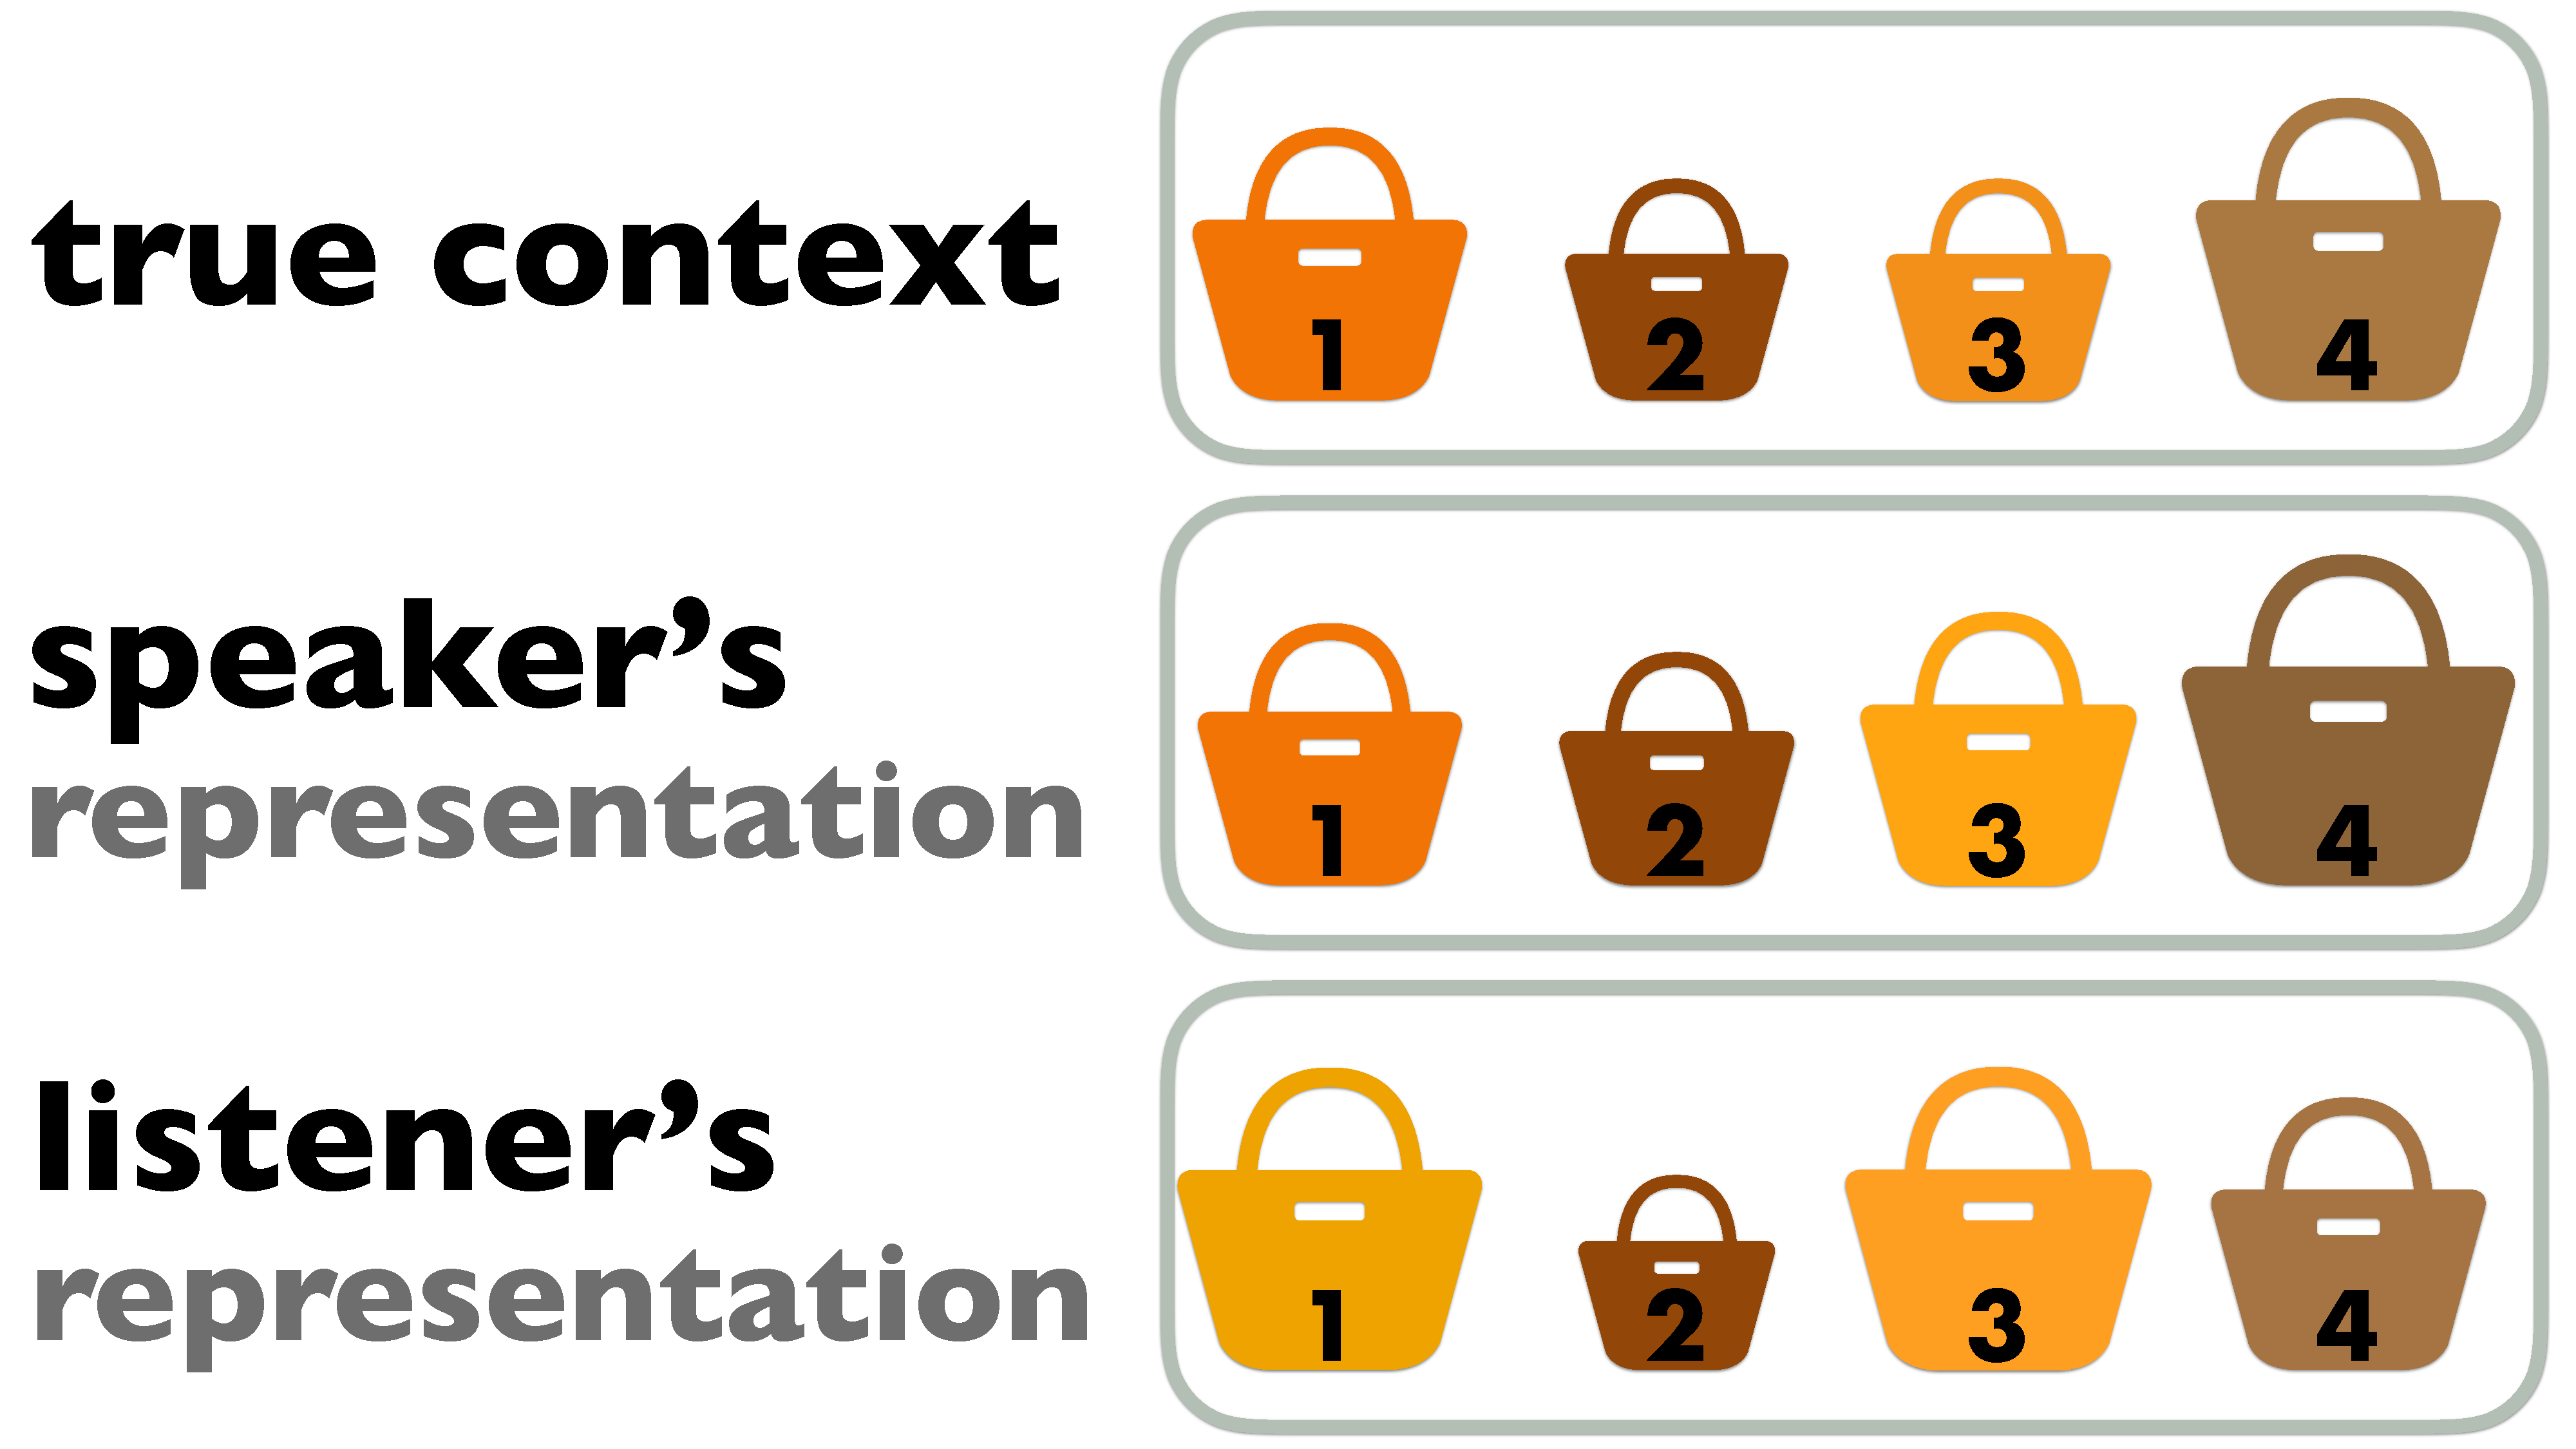
\includegraphics[width=\linewidth]{model_picture.pdf} 
  \caption{Illustration of the model}
  \label{fig:ModelIllustration}
\end{figure}

\bibliographystyle{apacite}
\setlength{\bibleftmargin}{.125in}
\setlength{\bibindent}{-\bibleftmargin}

\bibliography{adjOrder}

\end{document}

